% Options for packages loaded elsewhere
\PassOptionsToPackage{unicode}{hyperref}
\PassOptionsToPackage{hyphens}{url}
\PassOptionsToPackage{dvipsnames,svgnames,x11names}{xcolor}
%
\documentclass[
  letterpaper,
  DIV=11,
  numbers=noendperiod]{scrreprt}

\usepackage{amsmath,amssymb}
\usepackage{iftex}
\ifPDFTeX
  \usepackage[T1]{fontenc}
  \usepackage[utf8]{inputenc}
  \usepackage{textcomp} % provide euro and other symbols
\else % if luatex or xetex
  \usepackage{unicode-math}
  \defaultfontfeatures{Scale=MatchLowercase}
  \defaultfontfeatures[\rmfamily]{Ligatures=TeX,Scale=1}
\fi
\usepackage{lmodern}
\ifPDFTeX\else  
    % xetex/luatex font selection
\fi
% Use upquote if available, for straight quotes in verbatim environments
\IfFileExists{upquote.sty}{\usepackage{upquote}}{}
\IfFileExists{microtype.sty}{% use microtype if available
  \usepackage[]{microtype}
  \UseMicrotypeSet[protrusion]{basicmath} % disable protrusion for tt fonts
}{}
\makeatletter
\@ifundefined{KOMAClassName}{% if non-KOMA class
  \IfFileExists{parskip.sty}{%
    \usepackage{parskip}
  }{% else
    \setlength{\parindent}{0pt}
    \setlength{\parskip}{6pt plus 2pt minus 1pt}}
}{% if KOMA class
  \KOMAoptions{parskip=half}}
\makeatother
\usepackage{xcolor}
\setlength{\emergencystretch}{3em} % prevent overfull lines
\setcounter{secnumdepth}{3}
% Make \paragraph and \subparagraph free-standing
\ifx\paragraph\undefined\else
  \let\oldparagraph\paragraph
  \renewcommand{\paragraph}[1]{\oldparagraph{#1}\mbox{}}
\fi
\ifx\subparagraph\undefined\else
  \let\oldsubparagraph\subparagraph
  \renewcommand{\subparagraph}[1]{\oldsubparagraph{#1}\mbox{}}
\fi

\usepackage{color}
\usepackage{fancyvrb}
\newcommand{\VerbBar}{|}
\newcommand{\VERB}{\Verb[commandchars=\\\{\}]}
\DefineVerbatimEnvironment{Highlighting}{Verbatim}{commandchars=\\\{\}}
% Add ',fontsize=\small' for more characters per line
\usepackage{framed}
\definecolor{shadecolor}{RGB}{241,243,245}
\newenvironment{Shaded}{\begin{snugshade}}{\end{snugshade}}
\newcommand{\AlertTok}[1]{\textcolor[rgb]{0.68,0.00,0.00}{#1}}
\newcommand{\AnnotationTok}[1]{\textcolor[rgb]{0.37,0.37,0.37}{#1}}
\newcommand{\AttributeTok}[1]{\textcolor[rgb]{0.40,0.45,0.13}{#1}}
\newcommand{\BaseNTok}[1]{\textcolor[rgb]{0.68,0.00,0.00}{#1}}
\newcommand{\BuiltInTok}[1]{\textcolor[rgb]{0.00,0.23,0.31}{#1}}
\newcommand{\CharTok}[1]{\textcolor[rgb]{0.13,0.47,0.30}{#1}}
\newcommand{\CommentTok}[1]{\textcolor[rgb]{0.37,0.37,0.37}{#1}}
\newcommand{\CommentVarTok}[1]{\textcolor[rgb]{0.37,0.37,0.37}{\textit{#1}}}
\newcommand{\ConstantTok}[1]{\textcolor[rgb]{0.56,0.35,0.01}{#1}}
\newcommand{\ControlFlowTok}[1]{\textcolor[rgb]{0.00,0.23,0.31}{#1}}
\newcommand{\DataTypeTok}[1]{\textcolor[rgb]{0.68,0.00,0.00}{#1}}
\newcommand{\DecValTok}[1]{\textcolor[rgb]{0.68,0.00,0.00}{#1}}
\newcommand{\DocumentationTok}[1]{\textcolor[rgb]{0.37,0.37,0.37}{\textit{#1}}}
\newcommand{\ErrorTok}[1]{\textcolor[rgb]{0.68,0.00,0.00}{#1}}
\newcommand{\ExtensionTok}[1]{\textcolor[rgb]{0.00,0.23,0.31}{#1}}
\newcommand{\FloatTok}[1]{\textcolor[rgb]{0.68,0.00,0.00}{#1}}
\newcommand{\FunctionTok}[1]{\textcolor[rgb]{0.28,0.35,0.67}{#1}}
\newcommand{\ImportTok}[1]{\textcolor[rgb]{0.00,0.46,0.62}{#1}}
\newcommand{\InformationTok}[1]{\textcolor[rgb]{0.37,0.37,0.37}{#1}}
\newcommand{\KeywordTok}[1]{\textcolor[rgb]{0.00,0.23,0.31}{#1}}
\newcommand{\NormalTok}[1]{\textcolor[rgb]{0.00,0.23,0.31}{#1}}
\newcommand{\OperatorTok}[1]{\textcolor[rgb]{0.37,0.37,0.37}{#1}}
\newcommand{\OtherTok}[1]{\textcolor[rgb]{0.00,0.23,0.31}{#1}}
\newcommand{\PreprocessorTok}[1]{\textcolor[rgb]{0.68,0.00,0.00}{#1}}
\newcommand{\RegionMarkerTok}[1]{\textcolor[rgb]{0.00,0.23,0.31}{#1}}
\newcommand{\SpecialCharTok}[1]{\textcolor[rgb]{0.37,0.37,0.37}{#1}}
\newcommand{\SpecialStringTok}[1]{\textcolor[rgb]{0.13,0.47,0.30}{#1}}
\newcommand{\StringTok}[1]{\textcolor[rgb]{0.13,0.47,0.30}{#1}}
\newcommand{\VariableTok}[1]{\textcolor[rgb]{0.07,0.07,0.07}{#1}}
\newcommand{\VerbatimStringTok}[1]{\textcolor[rgb]{0.13,0.47,0.30}{#1}}
\newcommand{\WarningTok}[1]{\textcolor[rgb]{0.37,0.37,0.37}{\textit{#1}}}

\providecommand{\tightlist}{%
  \setlength{\itemsep}{0pt}\setlength{\parskip}{0pt}}\usepackage{longtable,booktabs,array}
\usepackage{calc} % for calculating minipage widths
% Correct order of tables after \paragraph or \subparagraph
\usepackage{etoolbox}
\makeatletter
\patchcmd\longtable{\par}{\if@noskipsec\mbox{}\fi\par}{}{}
\makeatother
% Allow footnotes in longtable head/foot
\IfFileExists{footnotehyper.sty}{\usepackage{footnotehyper}}{\usepackage{footnote}}
\makesavenoteenv{longtable}
\usepackage{graphicx}
\makeatletter
\def\maxwidth{\ifdim\Gin@nat@width>\linewidth\linewidth\else\Gin@nat@width\fi}
\def\maxheight{\ifdim\Gin@nat@height>\textheight\textheight\else\Gin@nat@height\fi}
\makeatother
% Scale images if necessary, so that they will not overflow the page
% margins by default, and it is still possible to overwrite the defaults
% using explicit options in \includegraphics[width, height, ...]{}
\setkeys{Gin}{width=\maxwidth,height=\maxheight,keepaspectratio}
% Set default figure placement to htbp
\makeatletter
\def\fps@figure{htbp}
\makeatother
% definitions for citeproc citations
\NewDocumentCommand\citeproctext{}{}
\NewDocumentCommand\citeproc{mm}{%
  \begingroup\def\citeproctext{#2}\cite{#1}\endgroup}
\makeatletter
 % allow citations to break across lines
 \let\@cite@ofmt\@firstofone
 % avoid brackets around text for \cite:
 \def\@biblabel#1{}
 \def\@cite#1#2{{#1\if@tempswa , #2\fi}}
\makeatother
\newlength{\cslhangindent}
\setlength{\cslhangindent}{1.5em}
\newlength{\csllabelwidth}
\setlength{\csllabelwidth}{3em}
\newenvironment{CSLReferences}[2] % #1 hanging-indent, #2 entry-spacing
 {\begin{list}{}{%
  \setlength{\itemindent}{0pt}
  \setlength{\leftmargin}{0pt}
  \setlength{\parsep}{0pt}
  % turn on hanging indent if param 1 is 1
  \ifodd #1
   \setlength{\leftmargin}{\cslhangindent}
   \setlength{\itemindent}{-1\cslhangindent}
  \fi
  % set entry spacing
  \setlength{\itemsep}{#2\baselineskip}}}
 {\end{list}}
\usepackage{calc}
\newcommand{\CSLBlock}[1]{\hfill\break\parbox[t]{\linewidth}{\strut\ignorespaces#1\strut}}
\newcommand{\CSLLeftMargin}[1]{\parbox[t]{\csllabelwidth}{\strut#1\strut}}
\newcommand{\CSLRightInline}[1]{\parbox[t]{\linewidth - \csllabelwidth}{\strut#1\strut}}
\newcommand{\CSLIndent}[1]{\hspace{\cslhangindent}#1}

% Soul package to handle highlighting (see hl.py3 filter)
\usepackage{soul}

\usepackage{booktabs}
\usepackage{longtable}
\usepackage{array}
\usepackage{multirow}
\usepackage{wrapfig}
\usepackage{float}
\usepackage{colortbl}
\usepackage{pdflscape}
\usepackage{tabu}
\usepackage{threeparttable}
\usepackage{threeparttablex}
\usepackage[normalem]{ulem}
\usepackage{makecell}
\usepackage{xcolor}
\usepackage{caption}
\KOMAoption{captions}{tableheading}
\makeatletter
\@ifpackageloaded{tcolorbox}{}{\usepackage[skins,breakable]{tcolorbox}}
\@ifpackageloaded{fontawesome5}{}{\usepackage{fontawesome5}}
\definecolor{quarto-callout-color}{HTML}{909090}
\definecolor{quarto-callout-note-color}{HTML}{0758E5}
\definecolor{quarto-callout-important-color}{HTML}{CC1914}
\definecolor{quarto-callout-warning-color}{HTML}{EB9113}
\definecolor{quarto-callout-tip-color}{HTML}{00A047}
\definecolor{quarto-callout-caution-color}{HTML}{FC5300}
\definecolor{quarto-callout-color-frame}{HTML}{acacac}
\definecolor{quarto-callout-note-color-frame}{HTML}{4582ec}
\definecolor{quarto-callout-important-color-frame}{HTML}{d9534f}
\definecolor{quarto-callout-warning-color-frame}{HTML}{f0ad4e}
\definecolor{quarto-callout-tip-color-frame}{HTML}{02b875}
\definecolor{quarto-callout-caution-color-frame}{HTML}{fd7e14}
\makeatother
\makeatletter
\@ifpackageloaded{bookmark}{}{\usepackage{bookmark}}
\makeatother
\makeatletter
\@ifpackageloaded{caption}{}{\usepackage{caption}}
\AtBeginDocument{%
\ifdefined\contentsname
  \renewcommand*\contentsname{Índice}
\else
  \newcommand\contentsname{Índice}
\fi
\ifdefined\listfigurename
  \renewcommand*\listfigurename{Lista de Figuras}
\else
  \newcommand\listfigurename{Lista de Figuras}
\fi
\ifdefined\listtablename
  \renewcommand*\listtablename{Lista de Tabelas}
\else
  \newcommand\listtablename{Lista de Tabelas}
\fi
\ifdefined\figurename
  \renewcommand*\figurename{Figura}
\else
  \newcommand\figurename{Figura}
\fi
\ifdefined\tablename
  \renewcommand*\tablename{Tabela}
\else
  \newcommand\tablename{Tabela}
\fi
}
\@ifpackageloaded{float}{}{\usepackage{float}}
\floatstyle{ruled}
\@ifundefined{c@chapter}{\newfloat{codelisting}{h}{lop}}{\newfloat{codelisting}{h}{lop}[chapter]}
\floatname{codelisting}{Listagem}
\newcommand*\listoflistings{\listof{codelisting}{Lista de Listagens}}
\makeatother
\makeatletter
\makeatother
\makeatletter
\@ifpackageloaded{caption}{}{\usepackage{caption}}
\@ifpackageloaded{subcaption}{}{\usepackage{subcaption}}
\makeatother
\ifLuaTeX
\usepackage[bidi=basic]{babel}
\else
\usepackage[bidi=default]{babel}
\fi
\babelprovide[main,import]{portuguese}
% get rid of language-specific shorthands (see #6817):
\let\LanguageShortHands\languageshorthands
\def\languageshorthands#1{}
\ifLuaTeX
  \usepackage{selnolig}  % disable illegal ligatures
\fi
\usepackage{bookmark}

\IfFileExists{xurl.sty}{\usepackage{xurl}}{} % add URL line breaks if available
\urlstyle{same} % disable monospaced font for URLs
\hypersetup{
  pdftitle={Regressão Linear},
  pdfauthor={Fernando Náufel},
  pdflang={pt},
  colorlinks=true,
  linkcolor={blue},
  filecolor={Maroon},
  citecolor={Blue},
  urlcolor={Blue},
  pdfcreator={LaTeX via pandoc}}

\title{Regressão Linear}
\author{Fernando Náufel}
\date{03/05/2024 18:22}

\begin{document}
\maketitle

% Bold title in callout boxes
\tcbset{fonttitle=\bfseries}

\renewcommand*\contentsname{Índice}
{
\hypersetup{linkcolor=}
\setcounter{tocdepth}{2}
\tableofcontents
}
\bookmarksetup{startatroot}

\chapter*{Apresentação}\label{apresentauxe7uxe3o}
\addcontentsline{toc}{chapter}{Apresentação}

\markboth{Apresentação}{Apresentação}

???

\bookmarksetup{startatroot}

\chapter{Regressão linear simples}\label{regressuxe3o-linear-simples}

\section{Exemplo: vendas e
publicidade}\label{exemplo-vendas-e-publicidade}

Exemplo baseado no livro James et al. (2021), com dados obtidos de
\url{https://www.kaggle.com/datasets/ashydv/advertising-dataset/data}.

Este conjunto de dados contém $4$ colunas:

\begin{itemize}
\tightlist
\item
  \texttt{tv}: verba (em milhares de dólares) gasta em publicidade na
  TV;
\item
  \texttt{radio}: verba (em milhares de dólares) gasta em publicidade no
  rádio;
\item
  \texttt{jornal}: verba (em milhares de dólares) gasta em publicidade
  em jornais;
\item
  \texttt{vendas}: receita das vendas (em milhares de dólares).
\end{itemize}

Cada observação --- isto é, cada linha --- corresponde a um produto.

\subsection{Leitura e limpeza}\label{leitura-e-limpeza}

\begin{Shaded}
\begin{Highlighting}[]
\NormalTok{publicidade }\OtherTok{\textless{}{-}} \FunctionTok{read\_csv}\NormalTok{(}
  \StringTok{\textquotesingle{}dados/advertising.csv\textquotesingle{}}\NormalTok{,}
  \AttributeTok{show\_col\_types =} \ConstantTok{FALSE}
\NormalTok{) }\SpecialCharTok{\%\textgreater{}\%} 
\NormalTok{  janitor}\SpecialCharTok{::}\FunctionTok{clean\_names}\NormalTok{() }\SpecialCharTok{\%\textgreater{}\%} 
  \FunctionTok{rename}\NormalTok{(}
    \AttributeTok{jornal =}\NormalTok{ newspaper,}
    \AttributeTok{vendas =}\NormalTok{ sales}
\NormalTok{  )}

\NormalTok{publicidade }\SpecialCharTok{\%\textgreater{}\%} \FunctionTok{gt}\NormalTok{()}
\end{Highlighting}
\end{Shaded}

\begin{longtable*}{rrrr}
\toprule
tv & radio & jornal & vendas \\ 
\midrule\addlinespace[2.5pt]
230,1 & 37,8 & 69,2 & 22,1 \\ 
44,5 & 39,3 & 45,1 & 10,4 \\ 
17,2 & 45,9 & 69,3 & 12,0 \\ 
151,5 & 41,3 & 58,5 & 16,5 \\ 
180,8 & 10,8 & 58,4 & 17,9 \\ 
8,7 & 48,9 & 75,0 & 7,2 \\ 
57,5 & 32,8 & 23,5 & 11,8 \\ 
120,2 & 19,6 & 11,6 & 13,2 \\ 
8,6 & 2,1 & 1,0 & 4,8 \\ 
199,8 & 2,6 & 21,2 & 15,6 \\ 
66,1 & 5,8 & 24,2 & 12,6 \\ 
214,7 & 24,0 & 4,0 & 17,4 \\ 
23,8 & 35,1 & 65,9 & 9,2 \\ 
97,5 & 7,6 & 7,2 & 13,7 \\ 
204,1 & 32,9 & 46,0 & 19,0 \\ 
195,4 & 47,7 & 52,9 & 22,4 \\ 
67,8 & 36,6 & 114,0 & 12,5 \\ 
281,4 & 39,6 & 55,8 & 24,4 \\ 
69,2 & 20,5 & 18,3 & 11,3 \\ 
147,3 & 23,9 & 19,1 & 14,6 \\ 
218,4 & 27,7 & 53,4 & 18,0 \\ 
237,4 & 5,1 & 23,5 & 17,5 \\ 
13,2 & 15,9 & 49,6 & 5,6 \\ 
228,3 & 16,9 & 26,2 & 20,5 \\ 
62,3 & 12,6 & 18,3 & 9,7 \\ 
262,9 & 3,5 & 19,5 & 17,0 \\ 
142,9 & 29,3 & 12,6 & 15,0 \\ 
240,1 & 16,7 & 22,9 & 20,9 \\ 
248,8 & 27,1 & 22,9 & 18,9 \\ 
70,6 & 16,0 & 40,8 & 10,5 \\ 
292,9 & 28,3 & 43,2 & 21,4 \\ 
112,9 & 17,4 & 38,6 & 11,9 \\ 
97,2 & 1,5 & 30,0 & 13,2 \\ 
265,6 & 20,0 & 0,3 & 17,4 \\ 
95,7 & 1,4 & 7,4 & 11,9 \\ 
290,7 & 4,1 & 8,5 & 17,8 \\ 
266,9 & 43,8 & 5,0 & 25,4 \\ 
74,7 & 49,4 & 45,7 & 14,7 \\ 
43,1 & 26,7 & 35,1 & 10,1 \\ 
228,0 & 37,7 & 32,0 & 21,5 \\ 
202,5 & 22,3 & 31,6 & 16,6 \\ 
177,0 & 33,4 & 38,7 & 17,1 \\ 
293,6 & 27,7 & 1,8 & 20,7 \\ 
206,9 & 8,4 & 26,4 & 17,9 \\ 
25,1 & 25,7 & 43,3 & 8,5 \\ 
175,1 & 22,5 & 31,5 & 16,1 \\ 
89,7 & 9,9 & 35,7 & 10,6 \\ 
239,9 & 41,5 & 18,5 & 23,2 \\ 
227,2 & 15,8 & 49,9 & 19,8 \\ 
66,9 & 11,7 & 36,8 & 9,7 \\ 
199,8 & 3,1 & 34,6 & 16,4 \\ 
100,4 & 9,6 & 3,6 & 10,7 \\ 
216,4 & 41,7 & 39,6 & 22,6 \\ 
182,6 & 46,2 & 58,7 & 21,2 \\ 
262,7 & 28,8 & 15,9 & 20,2 \\ 
198,9 & 49,4 & 60,0 & 23,7 \\ 
7,3 & 28,1 & 41,4 & 5,5 \\ 
136,2 & 19,2 & 16,6 & 13,2 \\ 
210,8 & 49,6 & 37,7 & 23,8 \\ 
210,7 & 29,5 & 9,3 & 18,4 \\ 
53,5 & 2,0 & 21,4 & 8,1 \\ 
261,3 & 42,7 & 54,7 & 24,2 \\ 
239,3 & 15,5 & 27,3 & 20,7 \\ 
102,7 & 29,6 & 8,4 & 14,0 \\ 
131,1 & 42,8 & 28,9 & 16,0 \\ 
69,0 & 9,3 & 0,9 & 11,3 \\ 
31,5 & 24,6 & 2,2 & 11,0 \\ 
139,3 & 14,5 & 10,2 & 13,4 \\ 
237,4 & 27,5 & 11,0 & 18,9 \\ 
216,8 & 43,9 & 27,2 & 22,3 \\ 
199,1 & 30,6 & 38,7 & 18,3 \\ 
109,8 & 14,3 & 31,7 & 12,4 \\ 
26,8 & 33,0 & 19,3 & 8,8 \\ 
129,4 & 5,7 & 31,3 & 11,0 \\ 
213,4 & 24,6 & 13,1 & 17,0 \\ 
16,9 & 43,7 & 89,4 & 8,7 \\ 
27,5 & 1,6 & 20,7 & 6,9 \\ 
120,5 & 28,5 & 14,2 & 14,2 \\ 
5,4 & 29,9 & 9,4 & 5,3 \\ 
116,0 & 7,7 & 23,1 & 11,0 \\ 
76,4 & 26,7 & 22,3 & 11,8 \\ 
239,8 & 4,1 & 36,9 & 17,3 \\ 
75,3 & 20,3 & 32,5 & 11,3 \\ 
68,4 & 44,5 & 35,6 & 13,6 \\ 
213,5 & 43,0 & 33,8 & 21,7 \\ 
193,2 & 18,4 & 65,7 & 20,2 \\ 
76,3 & 27,5 & 16,0 & 12,0 \\ 
110,7 & 40,6 & 63,2 & 16,0 \\ 
88,3 & 25,5 & 73,4 & 12,9 \\ 
109,8 & 47,8 & 51,4 & 16,7 \\ 
134,3 & 4,9 & 9,3 & 14,0 \\ 
28,6 & 1,5 & 33,0 & 7,3 \\ 
217,7 & 33,5 & 59,0 & 19,4 \\ 
250,9 & 36,5 & 72,3 & 22,2 \\ 
107,4 & 14,0 & 10,9 & 11,5 \\ 
163,3 & 31,6 & 52,9 & 16,9 \\ 
197,6 & 3,5 & 5,9 & 16,7 \\ 
184,9 & 21,0 & 22,0 & 20,5 \\ 
289,7 & 42,3 & 51,2 & 25,4 \\ 
135,2 & 41,7 & 45,9 & 17,2 \\ 
222,4 & 4,3 & 49,8 & 16,7 \\ 
296,4 & 36,3 & 100,9 & 23,8 \\ 
280,2 & 10,1 & 21,4 & 19,8 \\ 
187,9 & 17,2 & 17,9 & 19,7 \\ 
238,2 & 34,3 & 5,3 & 20,7 \\ 
137,9 & 46,4 & 59,0 & 15,0 \\ 
25,0 & 11,0 & 29,7 & 7,2 \\ 
90,4 & 0,3 & 23,2 & 12,0 \\ 
13,1 & 0,4 & 25,6 & 5,3 \\ 
255,4 & 26,9 & 5,5 & 19,8 \\ 
225,8 & 8,2 & 56,5 & 18,4 \\ 
241,7 & 38,0 & 23,2 & 21,8 \\ 
175,7 & 15,4 & 2,4 & 17,1 \\ 
209,6 & 20,6 & 10,7 & 20,9 \\ 
78,2 & 46,8 & 34,5 & 14,6 \\ 
75,1 & 35,0 & 52,7 & 12,6 \\ 
139,2 & 14,3 & 25,6 & 12,2 \\ 
76,4 & 0,8 & 14,8 & 9,4 \\ 
125,7 & 36,9 & 79,2 & 15,9 \\ 
19,4 & 16,0 & 22,3 & 6,6 \\ 
141,3 & 26,8 & 46,2 & 15,5 \\ 
18,8 & 21,7 & 50,4 & 7,0 \\ 
224,0 & 2,4 & 15,6 & 16,6 \\ 
123,1 & 34,6 & 12,4 & 15,2 \\ 
229,5 & 32,3 & 74,2 & 19,7 \\ 
87,2 & 11,8 & 25,9 & 10,6 \\ 
7,8 & 38,9 & 50,6 & 6,6 \\ 
80,2 & 0,0 & 9,2 & 11,9 \\ 
220,3 & 49,0 & 3,2 & 24,7 \\ 
59,6 & 12,0 & 43,1 & 9,7 \\ 
0,7 & 39,6 & 8,7 & 1,6 \\ 
265,2 & 2,9 & 43,0 & 17,7 \\ 
8,4 & 27,2 & 2,1 & 5,7 \\ 
219,8 & 33,5 & 45,1 & 19,6 \\ 
36,9 & 38,6 & 65,6 & 10,8 \\ 
48,3 & 47,0 & 8,5 & 11,6 \\ 
25,6 & 39,0 & 9,3 & 9,5 \\ 
273,7 & 28,9 & 59,7 & 20,8 \\ 
43,0 & 25,9 & 20,5 & 9,6 \\ 
184,9 & 43,9 & 1,7 & 20,7 \\ 
73,4 & 17,0 & 12,9 & 10,9 \\ 
193,7 & 35,4 & 75,6 & 19,2 \\ 
220,5 & 33,2 & 37,9 & 20,1 \\ 
104,6 & 5,7 & 34,4 & 10,4 \\ 
96,2 & 14,8 & 38,9 & 12,3 \\ 
140,3 & 1,9 & 9,0 & 10,3 \\ 
240,1 & 7,3 & 8,7 & 18,2 \\ 
243,2 & 49,0 & 44,3 & 25,4 \\ 
38,0 & 40,3 & 11,9 & 10,9 \\ 
44,7 & 25,8 & 20,6 & 10,1 \\ 
280,7 & 13,9 & 37,0 & 16,1 \\ 
121,0 & 8,4 & 48,7 & 11,6 \\ 
197,6 & 23,3 & 14,2 & 16,6 \\ 
171,3 & 39,7 & 37,7 & 16,0 \\ 
187,8 & 21,1 & 9,5 & 20,6 \\ 
4,1 & 11,6 & 5,7 & 3,2 \\ 
93,9 & 43,5 & 50,5 & 15,3 \\ 
149,8 & 1,3 & 24,3 & 10,1 \\ 
11,7 & 36,9 & 45,2 & 7,3 \\ 
131,7 & 18,4 & 34,6 & 12,9 \\ 
172,5 & 18,1 & 30,7 & 16,4 \\ 
85,7 & 35,8 & 49,3 & 13,3 \\ 
188,4 & 18,1 & 25,6 & 19,9 \\ 
163,5 & 36,8 & 7,4 & 18,0 \\ 
117,2 & 14,7 & 5,4 & 11,9 \\ 
234,5 & 3,4 & 84,8 & 16,9 \\ 
17,9 & 37,6 & 21,6 & 8,0 \\ 
206,8 & 5,2 & 19,4 & 17,2 \\ 
215,4 & 23,6 & 57,6 & 17,1 \\ 
284,3 & 10,6 & 6,4 & 20,0 \\ 
50,0 & 11,6 & 18,4 & 8,4 \\ 
164,5 & 20,9 & 47,4 & 17,5 \\ 
19,6 & 20,1 & 17,0 & 7,6 \\ 
168,4 & 7,1 & 12,8 & 16,7 \\ 
222,4 & 3,4 & 13,1 & 16,5 \\ 
276,9 & 48,9 & 41,8 & 27,0 \\ 
248,4 & 30,2 & 20,3 & 20,2 \\ 
170,2 & 7,8 & 35,2 & 16,7 \\ 
276,7 & 2,3 & 23,7 & 16,8 \\ 
165,6 & 10,0 & 17,6 & 17,6 \\ 
156,6 & 2,6 & 8,3 & 15,5 \\ 
218,5 & 5,4 & 27,4 & 17,2 \\ 
56,2 & 5,7 & 29,7 & 8,7 \\ 
287,6 & 43,0 & 71,8 & 26,2 \\ 
253,8 & 21,3 & 30,0 & 17,6 \\ 
205,0 & 45,1 & 19,6 & 22,6 \\ 
139,5 & 2,1 & 26,6 & 10,3 \\ 
191,1 & 28,7 & 18,2 & 17,3 \\ 
286,0 & 13,9 & 3,7 & 20,9 \\ 
18,7 & 12,1 & 23,4 & 6,7 \\ 
39,5 & 41,1 & 5,8 & 10,8 \\ 
75,5 & 10,8 & 6,0 & 11,9 \\ 
17,2 & 4,1 & 31,6 & 5,9 \\ 
166,8 & 42,0 & 3,6 & 19,6 \\ 
149,7 & 35,6 & 6,0 & 17,3 \\ 
38,2 & 3,7 & 13,8 & 7,6 \\ 
94,2 & 4,9 & 8,1 & 14,0 \\ 
177,0 & 9,3 & 6,4 & 14,8 \\ 
283,6 & 42,0 & 66,2 & 25,5 \\ 
232,1 & 8,6 & 8,7 & 18,4 \\ 
\bottomrule
\end{longtable*}

\subsection{Divisão em dados de treino e
teste}\label{divisuxe3o-em-dados-de-treino-e-teste}

\begin{Shaded}
\begin{Highlighting}[]
\NormalTok{split }\OtherTok{\textless{}{-}} \FunctionTok{initial\_split}\NormalTok{(publicidade)}
\NormalTok{treino }\OtherTok{\textless{}{-}} \FunctionTok{training}\NormalTok{(split)}
\NormalTok{teste }\OtherTok{\textless{}{-}} \FunctionTok{testing}\NormalTok{(split)}
\NormalTok{split}
\end{Highlighting}
\end{Shaded}

\begin{verbatim}
<Training/Testing/Total>
<150/50/200>
\end{verbatim}

\subsection{Vendas por verba gasta em
TV}\label{vendas-por-verba-gasta-em-tv}

\subsubsection{Análise exploratória}\label{anuxe1lise-exploratuxf3ria}

Começamos visualizando os dados:

\begin{Shaded}
\begin{Highlighting}[]
\NormalTok{grafico }\OtherTok{\textless{}{-}}\NormalTok{ treino }\SpecialCharTok{\%\textgreater{}\%} 
  \FunctionTok{ggplot}\NormalTok{(}\FunctionTok{aes}\NormalTok{(tv, vendas)) }\SpecialCharTok{+}
    \FunctionTok{geom\_point}\NormalTok{()}

\NormalTok{grafico}
\end{Highlighting}
\end{Shaded}

\begin{center}
\includegraphics[width=1\textwidth,height=\textheight]{simples_files/figure-pdf/unnamed-chunk-4-1.pdf}
\end{center}

A correlação linear entre vendas e tv é

\begin{Shaded}
\begin{Highlighting}[]
\FunctionTok{cor}\NormalTok{(treino}\SpecialCharTok{$}\NormalTok{vendas, treino}\SpecialCharTok{$}\NormalTok{tv)}
\end{Highlighting}
\end{Shaded}

\begin{verbatim}
[1] 0,8919795
\end{verbatim}

\subsubsection{Modelo linear}\label{lm-vendas-tv}

\begin{Shaded}
\begin{Highlighting}[]
\NormalTok{modelo }\OtherTok{\textless{}{-}} \FunctionTok{lm}\NormalTok{(vendas }\SpecialCharTok{\textasciitilde{}}\NormalTok{ tv, }\AttributeTok{data =}\NormalTok{ treino)}
\FunctionTok{summary}\NormalTok{(modelo)}
\end{Highlighting}
\end{Shaded}

\begin{verbatim}

Call:
lm(formula = vendas ~ tv, data = treino)

Residuals:
    Min      1Q  Median      3Q     Max 
-6,0968 -1,5960 -0,0152  1,6301  5,2086 

Coefficients:
            Estimate Std. Error t value            Pr(>|t|)    
(Intercept) 7,185427   0,373754   19,23 <0,0000000000000002 ***
tv          0,053478   0,002228   24,00 <0,0000000000000002 ***
---
Signif. codes:  0 '***' 0,001 '**' 0,01 '*' 0,05 '.' 0,1 ' ' 1

Residual standard error: 2,289 on 148 degrees of freedom
Multiple R-squared:  0,7956,    Adjusted R-squared:  0,7942 
F-statistic: 576,2 on 1 and 148 DF,  p-value: < 0,00000000000000022
\end{verbatim}

\begin{Shaded}
\begin{Highlighting}[]
\NormalTok{modelo\_tidy }\OtherTok{\textless{}{-}} \FunctionTok{tidy}\NormalTok{(modelo)}
\NormalTok{modelo\_tidy}
\end{Highlighting}
\end{Shaded}

\begin{verbatim}
# A tibble: 2 x 5
  term        estimate std.error statistic  p.value
  <chr>          <dbl>     <dbl>     <dbl>    <dbl>
1 (Intercept)   7.19     0.374        19.2 4.49e-42
2 tv            0.0535   0.00223      24.0 6.86e-53
\end{verbatim}

\begin{Shaded}
\begin{Highlighting}[]
\NormalTok{b0 }\OtherTok{\textless{}{-}}\NormalTok{ modelo\_tidy}\SpecialCharTok{$}\NormalTok{estimate[}\DecValTok{1}\NormalTok{]}
\NormalTok{b1 }\OtherTok{\textless{}{-}}\NormalTok{ modelo\_tidy}\SpecialCharTok{$}\NormalTok{estimate[}\DecValTok{2}\NormalTok{]}
\end{Highlighting}
\end{Shaded}

\begin{Shaded}
\begin{Highlighting}[]
\NormalTok{grafico }\SpecialCharTok{+}
  \FunctionTok{geom\_abline}\NormalTok{(}
    \AttributeTok{intercept =}\NormalTok{ b0,}
    \AttributeTok{slope =}\NormalTok{ b1,}
    \AttributeTok{color =} \StringTok{\textquotesingle{}blue\textquotesingle{}}
\NormalTok{  )}
\end{Highlighting}
\end{Shaded}

\begin{center}
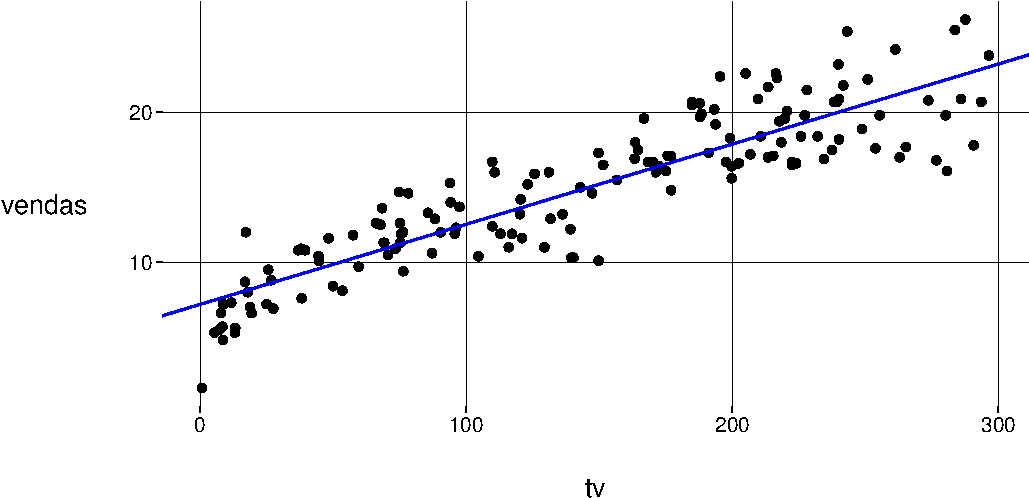
\includegraphics[width=1\textwidth,height=\textheight]{simples_files/figure-pdf/unnamed-chunk-9-1.pdf}
\end{center}

A equação da reta é

\[
\begin{aligned}
  \widehat{\text{vendas}} 
  &= \hat{\beta_0} + \hat{\beta_1} \cdot \text{tv} \\
  &= 7{,}19 + 0{,}05 \cdot \text{tv}
\end{aligned}
\]

\section{Teoria}\label{teoria}

\subsection{\texorpdfstring{Estimativas $\hat{\beta_0}$ e
$\hat{\beta_1}$}{Estimativas  e }}\label{estimativas-hatbeta_0-e-hatbeta_1}

Os valores achados são estimativas para $\beta_0$ e $\beta_1$, baseadas
nos dados do conjunto de treino.

Por isso, os valores de \texttt{vendas} obtidos com esta equação também
são estimativas.

Vamos escrever estimativas com o acento circunflexo (chapéu) sobre os
símbolos.

De onde vêm os valores de $\hat{\beta_0}$ e $\hat{\beta_1}$?

Resposta: são os valores que fazem com que a soma dos quadrados das
distâncias verticais dos pontos à reta seja a menor possível.

(Estas distâncias são chamadas de {\hl{resíduos}}.)

\href{https://fnaufel.github.io/probestr/regr.html\#como-achar-a-equa\%C3\%A7\%C3\%A3o-da-melhor-reta-com-c\%C3\%A1lculo}{Consulte
este material} para ver os detalhes sobre o cálculo de $\hat{\beta_0}$ e
$\hat{\beta_1}$.

\subsection{Erros-padrão das
estimativas}\label{erros-padruxe3o-das-estimativas}

Vamos pensar nas incertezas associadas aos valores de $\hat{\beta_0}$ e
$\hat{\beta_1}$, com base na excelente discussão em (De Veaux, Velleman
e Bock 2016, cap. 25).

Quais são os fatores que afetam a nossa confiança na reta de regressão?

Mais especificamente, {\hl{quais os fatores que afetam nossa confiança
no valor estimado $\hat\beta_1$}} (a inclinação da reta)?

\subsubsection{Espalhamento dos pontos em volta da
reta}\label{espalhamento-dos-pontos-em-volta-da-reta}

Quanto mais afastados da reta estiverem os dados, menor a nossa
confiança de que a reta captura a variação de uma variável em função da
outra.

Observe a Figura~\ref{fig-spread}. O gráfico da esquerda nos dá mais
certeza de que uma reta de regressão terá uma inclinação bem próxima da
taxa de variação de $y$ em função de $x$ na população.

\begin{figure}[htb]

\centering{

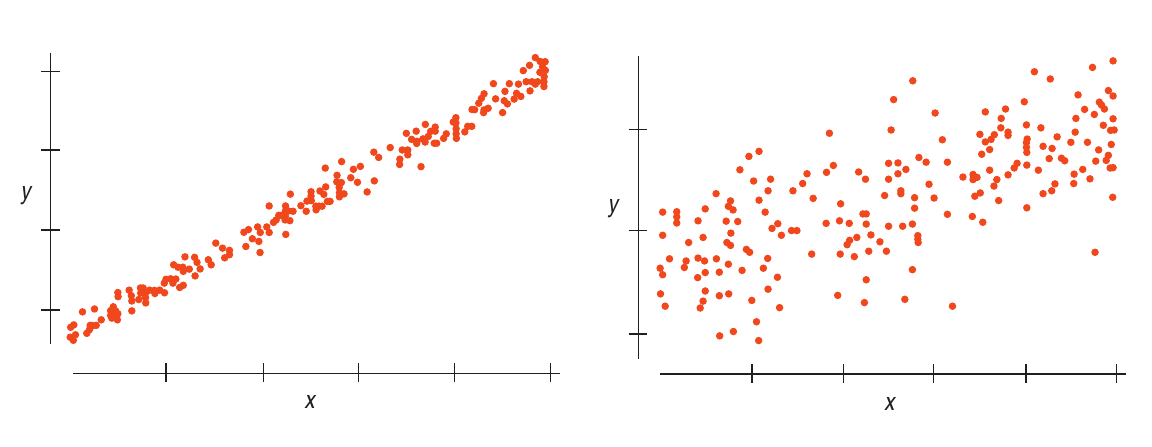
\includegraphics[width=1\textwidth,height=\textheight]{images/spread.png}

}

\caption{\label{fig-spread}Espalhamento dos pontos}

\end{figure}%

Este espalhamento é medido pelo {\hl{desvio-padrão dos resíduos}}.

\hyperref[lm-vendas-tv]{No exemplo das vendas}, este desvio-padrão dos
resíduos é calculado como

\[
\displaystyle
\sqrt{
\frac{\sum_i (\text{vendas}_i - \widehat{\text{vendas}}_i)^2}{n-2}
}
\]

No numerador, o valor $\text{vendas}_i - \widehat{\text{vendas}}_i$ é o
resíduo da observação $i$.

As \texttt{vendas} estimadas para cada valor de \texttt{tv} e os valores
dos resíduos podem ser acessados assim:

\begin{Shaded}
\begin{Highlighting}[]
\NormalTok{modelo\_augment }\OtherTok{\textless{}{-}} \FunctionTok{augment}\NormalTok{(modelo)}
\NormalTok{modelo\_augment }\SpecialCharTok{\%\textgreater{}\%} 
  \FunctionTok{select}\NormalTok{(vendas, tv, .fitted, .resid)}
\end{Highlighting}
\end{Shaded}

\begin{verbatim}
# A tibble: 150 x 4
  vendas    tv .fitted .resid
   <dbl> <dbl>   <dbl>  <dbl>
1   20.9 240.    20.0   0.874
2   11   116     13.4  -2.39 
3   10.1  44.7    9.58  0.524
4   16.7 222.    19.1  -2.38 
5   18.4 226.    19.3  -0.861
6    9.5  25.6    8.55  0.946
# i 144 more rows
\end{verbatim}

Calculando o desvio-padrão dos resíduos:

\begin{Shaded}
\begin{Highlighting}[]
\NormalTok{n }\OtherTok{\textless{}{-}} \FunctionTok{nrow}\NormalTok{(modelo\_augment)}
\NormalTok{dp\_residuos }\OtherTok{\textless{}{-}} \FunctionTok{sqrt}\NormalTok{(}\FunctionTok{sum}\NormalTok{(modelo\_augment}\SpecialCharTok{$}\NormalTok{.resid}\SpecialCharTok{\^{}}\DecValTok{2}\NormalTok{) }\SpecialCharTok{/}\NormalTok{ (n }\SpecialCharTok{{-}} \DecValTok{2}\NormalTok{))}
\NormalTok{dp\_residuos}
\end{Highlighting}
\end{Shaded}

\begin{verbatim}
[1] 2,28897
\end{verbatim}

Este valor pode ser obtido na coluna \texttt{sigma} do \emph{data frame}
retornado pela função \texttt{glance}:

\begin{Shaded}
\begin{Highlighting}[]
\NormalTok{modelo\_glance }\OtherTok{\textless{}{-}} \FunctionTok{glance}\NormalTok{(modelo)}
\NormalTok{modelo\_glance}\SpecialCharTok{$}\NormalTok{sigma}
\end{Highlighting}
\end{Shaded}

\begin{verbatim}
[1] 2,28897
\end{verbatim}

\begin{tcolorbox}[enhanced jigsaw, opacitybacktitle=0.6, titlerule=0mm, coltitle=black, bottomtitle=1mm, left=2mm, opacityback=0, bottomrule=.15mm, colframe=quarto-callout-important-color-frame, arc=.35mm, title=\textcolor{quarto-callout-important-color}{\faExclamation}\hspace{0.5em}{Desvio-padrão dos resíduos}, toprule=.15mm, colbacktitle=quarto-callout-important-color!10!white, toptitle=1mm, rightrule=.15mm, leftrule=.75mm, colback=white, breakable]

No geral, então, em uma regressão da variável $y$ sobre a variável $x$
com $n$ observações, o desvio-padrão dos resíduos é

\[
\displaystyle
s_{\text{residuos}} = 
\sqrt{
\frac{\sum_i (y_i - \widehat{y}_i)^2}{n-2}
}
\]

Pela Figura~\ref{fig-spread} e pelos comentários acima, quanto
{\hl{maior}} o valor de $s_{\text{residuos}}$, {\hl{maior}} a nossa
incerteza.

\end{tcolorbox}

\subsubsection{\texorpdfstring{Espalhamento de
$x$}{Espalhamento de }}\label{espalhamento-de-x}

Quanto maior o espalhamento dos valores de $x$, maior nossa confiança na
reta de regressão, pois ela estará baseada em uma diversidade maior de
valores.

Observe a Figura~\ref{fig-spread-x}. O gráfico da direita tem um
espalhamento maior dos valores de $x$. Uma reta de regressão, ali,
parece estar mais bem ``ancorada''.

\begin{figure}[htb]

\centering{

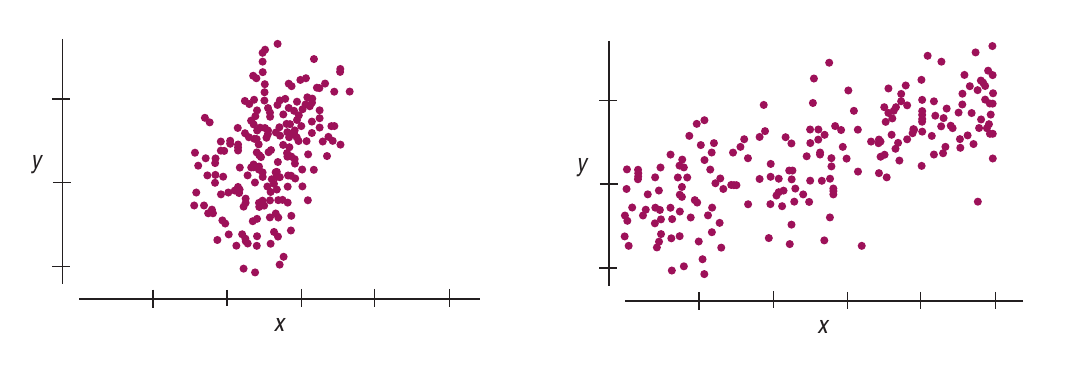
\includegraphics[width=1\textwidth,height=\textheight]{images/spread-x.png}

}

\caption{\label{fig-spread-x}Espalhamento de $x$}

\end{figure}%

O espalhamento de $x$ é medido pelo desvio-padrão, que é calculado da
maneira usual.

\hyperref[lm-vendas-tv]{No exemplo das vendas}, $s_x$, o desvio-padrão
de \texttt{tv} é

\begin{Shaded}
\begin{Highlighting}[]
\NormalTok{dp\_x }\OtherTok{\textless{}{-}}\NormalTok{ modelo\_augment }\SpecialCharTok{\%\textgreater{}\%} 
  \FunctionTok{pull}\NormalTok{(tv) }\SpecialCharTok{\%\textgreater{}\%} 
  \FunctionTok{sd}\NormalTok{()}

\NormalTok{dp\_x}
\end{Highlighting}
\end{Shaded}

\begin{verbatim}
[1] 84,16717
\end{verbatim}

\begin{tcolorbox}[enhanced jigsaw, opacitybacktitle=0.6, titlerule=0mm, coltitle=black, bottomtitle=1mm, left=2mm, opacityback=0, bottomrule=.15mm, colframe=quarto-callout-important-color-frame, arc=.35mm, title=\textcolor{quarto-callout-important-color}{\faExclamation}\hspace{0.5em}{Desvio-padrão dos resíduos}, toprule=.15mm, colbacktitle=quarto-callout-important-color!10!white, toptitle=1mm, rightrule=.15mm, leftrule=.75mm, colback=white, breakable]

Pela Figura~\ref{fig-spread-x} e pelos comentários acima, quanto
{\hl{maior}} o valor de $s_x$, {\hl{menor}} a nossa incerteza.

\end{tcolorbox}

\subsubsection{Quantidade de dados}\label{quantidade-de-dados}

Uma reta baseada em mais pontos é mais confiável. Observe a
Figura~\ref{fig-n}.

\begin{figure}[htb]

\centering{

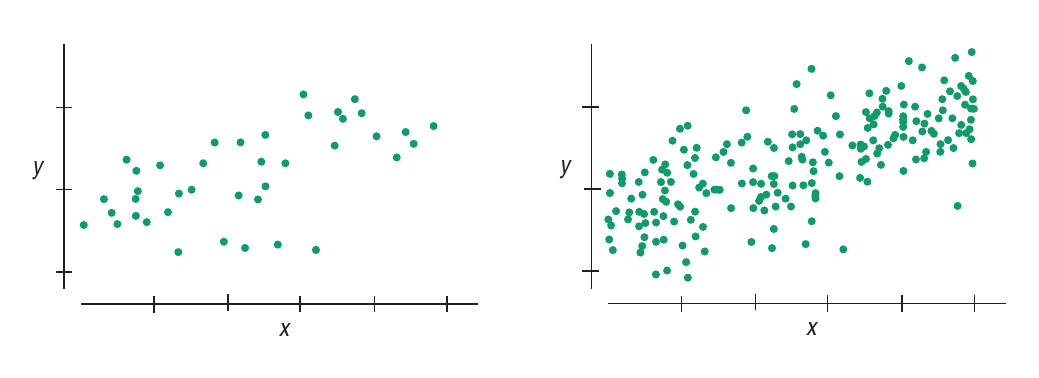
\includegraphics[width=1\textwidth,height=\textheight]{images/quantidade-dados.png}

}

\caption{\label{fig-n}Quantidade de dados}

\end{figure}%

\begin{tcolorbox}[enhanced jigsaw, opacitybacktitle=0.6, titlerule=0mm, coltitle=black, bottomtitle=1mm, left=2mm, opacityback=0, bottomrule=.15mm, colframe=quarto-callout-important-color-frame, arc=.35mm, title=\textcolor{quarto-callout-important-color}{\faExclamation}\hspace{0.5em}{Quantidade de dados}, toprule=.15mm, colbacktitle=quarto-callout-important-color!10!white, toptitle=1mm, rightrule=.15mm, leftrule=.75mm, colback=white, breakable]

Pela Figura~\ref{fig-n} e pelos comentários acima, quanto {\hl{maior}} o
valor de $n$, {\hl{menor}} a nossa incerteza.

\end{tcolorbox}

\subsubsection{Juntando tudo}\label{juntando-tudo}

Vimos que

\begin{itemize}
\tightlist
\item
  Quanto maior o desvio-padrão dos resíduos ($s_{\text{residuos}}$),
  {\hl{maior}} a incerteza.
\item
  Quanto maior o desvio-padrão da variável $x$ ($s_x$), {\hl{menor}} a
  incerteza.
\item
  Quanto maior a quantidade de dados ($n$), {\hl{menor}} a incerteza.
\end{itemize}

Concluímos que a incerteza sobre nossa estimativa para $\beta_1$ (a
inclinação da reta) é proporcional aos valores acima da seguinte
maneira:

\[
EP(\beta_1) \propto \frac{s_{\text{residuos}}}{n \cdot s_x}
\]

onde estamos escrevendo a incerteza como {\hl{$EP(\beta_1)$}}, o
{\hl{erro-padrão}} de $\beta_1$.

\begin{tcolorbox}[enhanced jigsaw, opacitybacktitle=0.6, titlerule=0mm, coltitle=black, bottomtitle=1mm, left=2mm, opacityback=0, bottomrule=.15mm, colframe=quarto-callout-important-color-frame, arc=.35mm, title=\textcolor{quarto-callout-important-color}{\faExclamation}\hspace{0.5em}{Erro-padrão de $\beta_1$}, toprule=.15mm, colbacktitle=quarto-callout-important-color!10!white, toptitle=1mm, rightrule=.15mm, leftrule=.75mm, colback=white, breakable]

A fórmula exata para a incerteza sobre $\beta_1$ é

\[
EP(\beta_1) = \frac{s_{\text{residuos}}}{\sqrt{n - 1} \cdot s_x}
\]

\end{tcolorbox}

\hyperref[lm-vendas-tv]{No exemplo das vendas}, usando as variáveis que
já calculamos antes, este erro-padrão é

\begin{Shaded}
\begin{Highlighting}[]
\NormalTok{dp\_residuos }\SpecialCharTok{/}\NormalTok{ (}\FunctionTok{sqrt}\NormalTok{(n }\SpecialCharTok{{-}} \DecValTok{1}\NormalTok{) }\SpecialCharTok{*}\NormalTok{ dp\_x)}
\end{Highlighting}
\end{Shaded}

\begin{verbatim}
[1] 0,002227943
\end{verbatim}

Este valor aparece nos resultados de \texttt{lm} como
\texttt{std.error}:

\begin{Shaded}
\begin{Highlighting}[]
\NormalTok{modelo\_tidy}
\end{Highlighting}
\end{Shaded}

\begin{verbatim}
# A tibble: 2 x 5
  term        estimate std.error statistic  p.value
  <chr>          <dbl>     <dbl>     <dbl>    <dbl>
1 (Intercept)   7.19     0.374        19.2 4.49e-42
2 tv            0.0535   0.00223      24.0 6.86e-53
\end{verbatim}

\subsubsection{Erro-padrão do
intercepto}\label{erro-padruxe3o-do-intercepto}

\begin{tcolorbox}[enhanced jigsaw, opacitybacktitle=0.6, titlerule=0mm, coltitle=black, bottomtitle=1mm, left=2mm, opacityback=0, bottomrule=.15mm, colframe=quarto-callout-important-color-frame, arc=.35mm, title=\textcolor{quarto-callout-important-color}{\faExclamation}\hspace{0.5em}{Erro-padrão de $\beta_0$}, toprule=.15mm, colbacktitle=quarto-callout-important-color!10!white, toptitle=1mm, rightrule=.15mm, leftrule=.75mm, colback=white, breakable]

Para o intercepto $\beta_0$, o raciocínio é análogo.

A fórmula exata para a incerteza sobre $\beta_0$ é

\[
EP(\beta_0) = 
\]

\end{tcolorbox}

??? ISLR p.~76

\section{Visão geométrica}\label{visuxe3o-geomuxe9trica}

Faraway (2016)

\subsection{Um pequeno exemplo}\label{um-pequeno-exemplo}

Para podermos visualizar a geometria, vamos considerar um conjunto de
dados com apenas $3$ observações.

A variável \texttt{x} é o único preditor, e a variável \texttt{y} é a
resposta.

\begin{Shaded}
\begin{Highlighting}[]
\NormalTok{df }\OtherTok{\textless{}{-}} \FunctionTok{tibble}\NormalTok{(}
  \AttributeTok{x =} \DecValTok{1}\SpecialCharTok{:}\DecValTok{3}\NormalTok{,}
  \AttributeTok{y =} \FunctionTok{c}\NormalTok{(}\DecValTok{4}\NormalTok{, }\DecValTok{3}\NormalTok{, }\DecValTok{8}\NormalTok{)}
\NormalTok{)}
\end{Highlighting}
\end{Shaded}

\begin{longtable*}{rr}
\toprule
x & y \\ 
\midrule\addlinespace[2.5pt]
1 & 4 \\ 
2 & 3 \\ 
3 & 8 \\ 
\bottomrule
\end{longtable*}

Graficamente:

\begin{center}
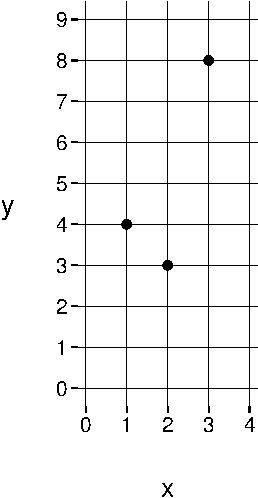
\includegraphics[width=1\textwidth,height=\textheight]{simples_files/figure-pdf/unnamed-chunk-18-1.pdf}
\end{center}

Com um único preditor, este é um exemplo de regressão simples. Queremos
achar uma equação da forma

\[
\hat y = \beta_0 + \beta_1x
\]

com valores de $\beta_0$ e $\beta_1$ que garantam a menor soma dos
quadrados dos resíduos.

Usamos o R para achar os coeficientes e outras informações sobre este
modelo:

\begin{Shaded}
\begin{Highlighting}[]
\NormalTok{modelo }\OtherTok{\textless{}{-}} \FunctionTok{lm}\NormalTok{(y }\SpecialCharTok{\textasciitilde{}}\NormalTok{ x, df)}
\FunctionTok{summary}\NormalTok{(modelo)}
\end{Highlighting}
\end{Shaded}

\begin{verbatim}

Call:
lm(formula = y ~ x, data = df)

Residuals:
 1  2  3 
 1 -2  1 

Coefficients:
            Estimate Std. Error t value Pr(>|t|)
(Intercept)    1,000      3,742   0,267    0,834
x              2,000      1,732   1,155    0,454

Residual standard error: 2,449 on 1 degrees of freedom
Multiple R-squared:  0,5714,    Adjusted R-squared:  0,1429 
F-statistic: 1,333 on 1 and 1 DF,  p-value: 0,4544
\end{verbatim}

A equação da reta que procuramos é

\[
\hat y = 1{,}00 + 2{,}00 x
\]

No gráfico, os valores de $\hat y$, para cada valor de $x$, são
mostrados em vermelho. A reta de regressão é mostrada em azul:

\begin{center}
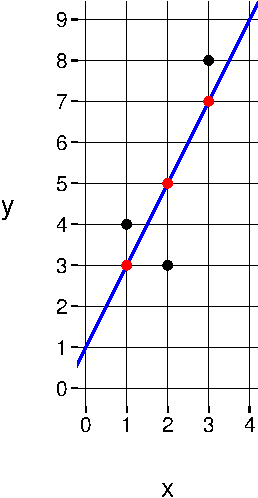
\includegraphics[width=1\textwidth,height=\textheight]{simples_files/figure-pdf/unnamed-chunk-21-1.pdf}
\end{center}

Os valores de $y$, os valores previstos e os resíduos são

\begin{longtable*}{rrrr}
\toprule
x & y & previsto & resíduo \\ 
\midrule\addlinespace[2.5pt]
1 & 4 & 3 & 1 \\ 
2 & 3 & 5 & -2 \\ 
3 & 8 & 7 & 1 \\ 
\bottomrule
\end{longtable*}

Usando Álgebra Linear, vamos encarar este modelo de outra forma.

A coluna \texttt{y} dos dados é representada pelo vetor

\[
\mathbf{Y} = \begin{bmatrix}
  4 \\ 3 \\ 8
\end{bmatrix}
\]

Vamos definir a seguinte matriz:

\[
\mathbf{X} = \begin{bmatrix}
  1 & 1 \\ 1 & 2 \\ 1 & 3
\end{bmatrix}
\]

Nesta matriz, a segunda coluna corresponde à coluna \texttt{x} dos
dados. A primeira coluna, com valores $1$, está ali para podermos
escrever o modelo como a equação matricial

\[
\mathbf{\widehat{Y}} = \mathbf{X} \cdot \begin{bmatrix}
  \beta_0 \\ \beta_1
\end{bmatrix}
\]

que, de forma mais detalhada, é

\[
\begin{bmatrix}
  \widehat{y_1} \\ \widehat{y_2} \\ \widehat{y_3}
\end{bmatrix}
=
\begin{bmatrix}
  1 & 1 \\ 1 & 2 \\ 1 & 3
\end{bmatrix}
\cdot \begin{bmatrix}
  \beta_0 \\ \beta_1
\end{bmatrix}
\]

ou, ainda,

\[
\begin{bmatrix}
  \widehat{y_1} \\ \widehat{y_2} \\ \widehat{y_3}
\end{bmatrix}
=
\begin{bmatrix}
  \beta_0 + \phantom{1\cdot{}}\beta_1 \\
  \beta_0 + 2\cdot \beta_1 \\
  \beta_0 + 3\cdot \beta_1
\end{bmatrix}
\]

ou, explicitando os vetores que correspondem às colunas da matriz
$\mathbf{X}$:

\begin{equation}\phantomsection\label{eq-modelo}{
\begin{bmatrix}
  \widehat{y_1} \\ \widehat{y_2} \\ \widehat{y_3}
\end{bmatrix}
=
\beta_0 \cdot 
\begin{bmatrix}
  1 \\ 1 \\ 1
\end{bmatrix}
+ 
\beta_1 \cdot
\begin{bmatrix}
  1 \\ 2 \\ 3
\end{bmatrix}
}\end{equation}

Agora, as considerações geométricas:

\begin{enumerate}
\def\labelenumi{\arabic{enumi}.}
\item
  As colunas \texttt{x} e \texttt{y} do conjunto de dados são vetores
  com $3$ componentes, que vivem em $\mathbb{R}^3$.
\item
  O vetor $\mathbf{\widehat Y}$ também tem $3$ componentes, mas a
  Equação~\ref{eq-modelo} está dizendo que $\mathbf{\widehat Y}$ é uma
  combinação linear dos dois vetores (linearmente independentes)
  $[1\ 1\ 1]^T$ e $[1\ 2\ 3]^T$.
\item
  Os dois vetores $[1\ 1\ 1]^T$ e $[1\ 2\ 3]^T$ não são capazes de gerar
  todo o espaço $\mathbb{R}^3$; o espaço gerado por eles é um plano.
\item
  O vetor $\mathbf{Y}$ (com os valores verdadeiros da variável de
  resposta $y$) não está no plano gerado pelos vetores $[1\ 1\ 1]^T$ e
  $[1\ 2\ 3]^T$ (verifique).
\item
  A relação verdadeira entre $\mathbf{Y}$ e $\mathbf{X}$ é

  \[
   \begin{bmatrix}
     y_1 \\ {y_2} \\ {y_3}
   \end{bmatrix}
   =
   \beta_0 \cdot 
   \begin{bmatrix}
     1 \\ 1 \\ 1
   \end{bmatrix}
   + 
   \beta_1 \cdot
   \begin{bmatrix}
     1 \\ 2 \\ 3
   \end{bmatrix}
   +
   \begin{bmatrix}
     \varepsilon_1 \\ \varepsilon_2 \\ \varepsilon_3
   \end{bmatrix}
  \] onde os valores $\varepsilon_i$ são os erros que o modelo não
  consegue capturar.
\item
  Estes erros $\varepsilon_i$ são estimados pelos resíduos
  $\widehat{\varepsilon_i}$, de maneira que podemos escrever

  \[
   \begin{bmatrix}
     \widehat{y_1} \\ \widehat{y_2} \\ \widehat{y_3}
   \end{bmatrix}
   =
   \beta_0 \cdot 
   \begin{bmatrix}
     1 \\ 1 \\ 1
   \end{bmatrix}
   + 
   \beta_1 \cdot
   \begin{bmatrix}
     1 \\ 2 \\ 3
   \end{bmatrix}
   +
   \begin{bmatrix}
     \widehat{\varepsilon_1} \\ 
     \widehat{\varepsilon_2} \\ 
     \widehat{\varepsilon_3}
   \end{bmatrix}
  \]

  O vetor de resíduos é

  \[
  \mathbf{\widehat{\varepsilon}} 
  = 
   \begin{bmatrix}
     \widehat{\varepsilon_1} \\ 
     \widehat{\varepsilon_2} \\ 
     \widehat{\varepsilon_3}
   \end{bmatrix}
   = 
   \begin{bmatrix}
      \phantom{-}1 \\ -2 \\ \phantom{-}1
   \end{bmatrix}
  \]
\end{enumerate}

A situação é mostrada na figura:

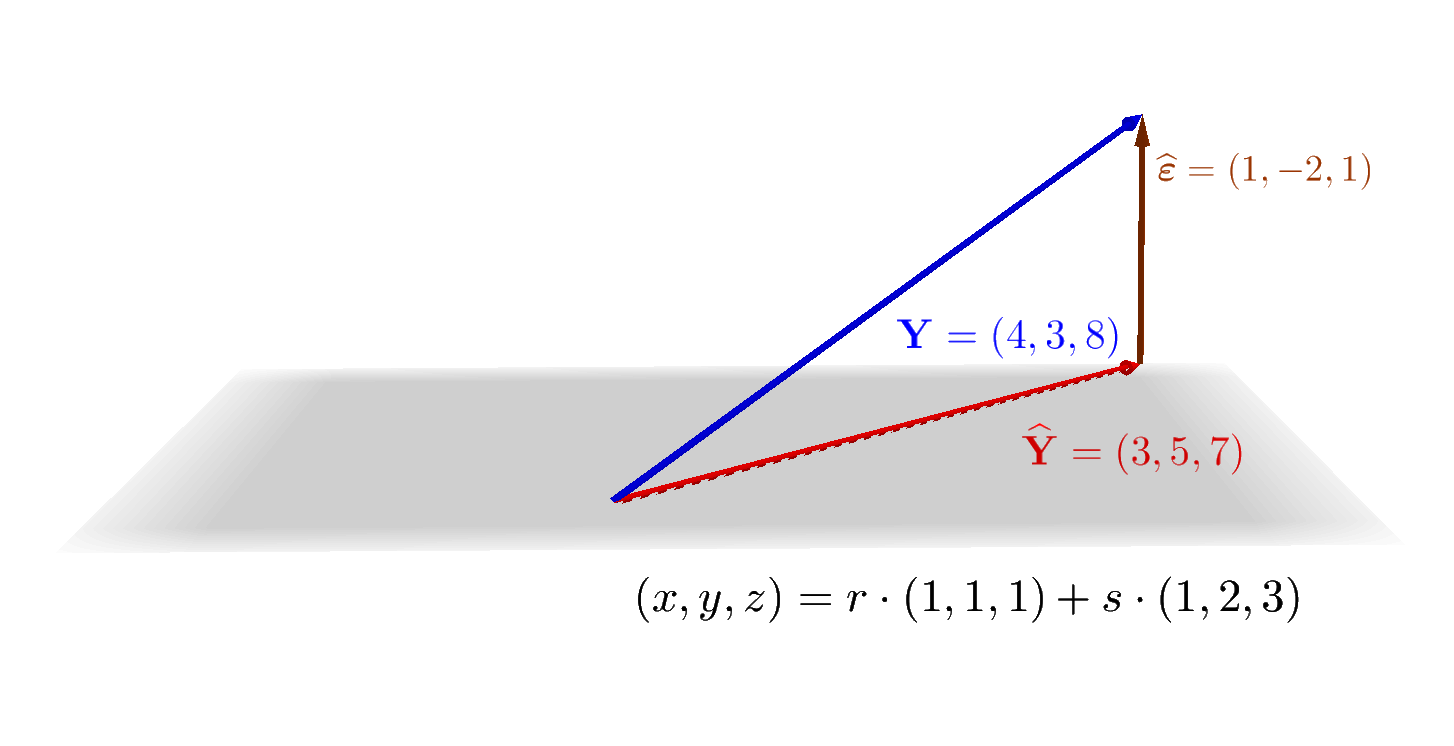
\includegraphics{images/regressao-visao-geometrica.png}

O plano cinza é o espaço gerado pelos vetores $[1\ 1\ 1]^T$ e
$[1\ 2\ 3]^T$. Na equação paramétrica deste plano, $r$ e $s$
correspondem aos valores possíveis de $\beta_0$ e $\beta_1$,
respectivamente.

O vetor $\mathbf{\widehat{Y}}$ (dos valores previstos pelo modelo) é a
projeção ortogonal do vetor $\mathbf{Y}$ (dos valores verdadeiros da
variável de resposta) sobre o plano gerado pelas colunas da matriz
$\mathbf{X}$. Mais abaixo, vamos ver os detalhes desta projeção. O
importante é entender que, quaisquer que sejam os valores de $\beta_0$ e
$\beta_1$, o vetor $\mathbf{\widehat{Y}}$ de valores previstos vai estar
sempre limitado ao plano gerado pelas colunas da matriz $\mathbf{X}$.

Isto corresponde à intuição de que estamos perdendo informação ao tentar
representar objetos de dimensão $3$ (o número de observações do conjunto
de dados) em um espaço de dimensão $2$ (o número de parâmetros do
modelo: $\beta_0$ e $\beta_1$).

???

\bookmarksetup{startatroot}

\chapter{Regressão linear
múltipla}\label{regressuxe3o-linear-muxfaltipla}

\section{Simulação}\label{simulauxe7uxe3o}

\subsection{Multicolinearidade}\label{multicolinearidade}

Vamos criar três preditores \texttt{x1}, \texttt{x2} e \texttt{x3}, com
os dois primeiros correlacionados:

\begin{Shaded}
\begin{Highlighting}[]
\NormalTok{n }\OtherTok{\textless{}{-}} \DecValTok{100}
\NormalTok{a }\OtherTok{\textless{}{-}} \DecValTok{2}
\NormalTok{x1 }\OtherTok{\textless{}{-}} \FunctionTok{runif}\NormalTok{(n)}
\NormalTok{x2 }\OtherTok{\textless{}{-}}\NormalTok{ a }\SpecialCharTok{*}\NormalTok{ x1 }\SpecialCharTok{+} \FunctionTok{rnorm}\NormalTok{(n, }\DecValTok{0}\NormalTok{, .}\DecValTok{1}\NormalTok{)}
\NormalTok{x3 }\OtherTok{\textless{}{-}} \FunctionTok{runif}\NormalTok{(n)}

\NormalTok{df }\OtherTok{\textless{}{-}} \FunctionTok{tibble}\NormalTok{(x1, x2, x3)}
\end{Highlighting}
\end{Shaded}

Gráficos:

\begin{Shaded}
\begin{Highlighting}[]
\NormalTok{plot\_cor }\OtherTok{\textless{}{-}} \ControlFlowTok{function}\NormalTok{(df, v1, v2) \{}
  
\NormalTok{  x }\OtherTok{=}\NormalTok{ df[[v1]]}
\NormalTok{  y }\OtherTok{=}\NormalTok{ df[[v2]]}
\NormalTok{  valor\_cor }\OtherTok{\textless{}{-}} \FunctionTok{cor}\NormalTok{(x, y) }\SpecialCharTok{\%\textgreater{}\%} \FunctionTok{round}\NormalTok{(}\DecValTok{4}\NormalTok{)}
  
\NormalTok{  df }\SpecialCharTok{\%\textgreater{}\%} \FunctionTok{ggplot}\NormalTok{(}\FunctionTok{aes}\NormalTok{(x, y)) }\SpecialCharTok{+}
    \FunctionTok{geom\_point}\NormalTok{(}\AttributeTok{alpha =} \FloatTok{0.5}\NormalTok{) }\SpecialCharTok{+}
    \FunctionTok{labs}\NormalTok{(}
      \AttributeTok{title =} \FunctionTok{paste0}\NormalTok{(}\StringTok{\textquotesingle{}cor(\textquotesingle{}}\NormalTok{, v1, }\StringTok{\textquotesingle{}, \textquotesingle{}}\NormalTok{, v2, }\StringTok{\textquotesingle{}) = \textquotesingle{}}\NormalTok{, valor\_cor),}
      \AttributeTok{x =}\NormalTok{ v1,}
      \AttributeTok{y =}\NormalTok{ v2}
\NormalTok{    )}
  
\NormalTok{\}}
\end{Highlighting}
\end{Shaded}

\begin{Shaded}
\begin{Highlighting}[]
\NormalTok{v }\OtherTok{\textless{}{-}} \FunctionTok{c}\NormalTok{(}\StringTok{\textquotesingle{}x1\textquotesingle{}}\NormalTok{, }\StringTok{\textquotesingle{}x2\textquotesingle{}}\NormalTok{, }\StringTok{\textquotesingle{}x3\textquotesingle{}}\NormalTok{)}

\NormalTok{pares }\OtherTok{\textless{}{-}} \FunctionTok{expand\_grid}\NormalTok{(}\AttributeTok{x =}\NormalTok{ v, }\AttributeTok{y =}\NormalTok{ v) }\SpecialCharTok{\%\textgreater{}\%} 
  \FunctionTok{filter}\NormalTok{(x }\SpecialCharTok{\textless{}}\NormalTok{ y) }\SpecialCharTok{\%\textgreater{}\%} 
  \FunctionTok{arrange}\NormalTok{(x, y)}

\NormalTok{v1 }\OtherTok{\textless{}{-}}\NormalTok{ pares }\SpecialCharTok{\%\textgreater{}\%} \FunctionTok{pull}\NormalTok{(x)}
\NormalTok{v2 }\OtherTok{\textless{}{-}}\NormalTok{ pares }\SpecialCharTok{\%\textgreater{}\%} \FunctionTok{pull}\NormalTok{(y)}

\NormalTok{plots }\OtherTok{\textless{}{-}} \FunctionTok{map2}\NormalTok{(}
\NormalTok{  v1, v2, }\SpecialCharTok{\textasciitilde{}} \FunctionTok{plot\_cor}\NormalTok{(df, .x, .y)}
\NormalTok{)}

\NormalTok{plots }\SpecialCharTok{\%\textgreater{}\%} 
  \FunctionTok{wrap\_plots}\NormalTok{(}
    \AttributeTok{ncol =} \DecValTok{1}\NormalTok{,}
    \AttributeTok{byrow =} \ConstantTok{TRUE}
\NormalTok{  )}
\end{Highlighting}
\end{Shaded}

\begin{center}
\includegraphics[width=1\textwidth,height=\textheight]{multipla_files/figure-pdf/unnamed-chunk-4-1.pdf}
\end{center}

A variável de resposta é \texttt{y}:

\begin{Shaded}
\begin{Highlighting}[]
\NormalTok{b0 }\OtherTok{\textless{}{-}} \DecValTok{1}
\NormalTok{b1 }\OtherTok{\textless{}{-}} \DecValTok{2}
\NormalTok{b2 }\OtherTok{\textless{}{-}} \DecValTok{3}
\NormalTok{b3 }\OtherTok{\textless{}{-}} \DecValTok{4}
\NormalTok{var\_epsilon }\OtherTok{\textless{}{-}}\NormalTok{ .}\DecValTok{5}

\NormalTok{y }\OtherTok{\textless{}{-}}\NormalTok{ b0 }\SpecialCharTok{+}\NormalTok{ b1 }\SpecialCharTok{*}\NormalTok{ x1 }\SpecialCharTok{+}\NormalTok{ b2 }\SpecialCharTok{*}\NormalTok{ x2 }\SpecialCharTok{+}\NormalTok{ b3 }\SpecialCharTok{*}\NormalTok{ x3 }\SpecialCharTok{+} \FunctionTok{rnorm}\NormalTok{(n, }\AttributeTok{sd =} \FunctionTok{sqrt}\NormalTok{(var\_epsilon))}
\NormalTok{df\_y }\OtherTok{\textless{}{-}}\NormalTok{ df }\SpecialCharTok{\%\textgreater{}\%} 
  \FunctionTok{mutate}\NormalTok{(}\AttributeTok{y =}\NormalTok{ y)}
\end{Highlighting}
\end{Shaded}

Usando todas as variáveis, temos:

\begin{Shaded}
\begin{Highlighting}[]
\NormalTok{modelo\_123 }\OtherTok{\textless{}{-}} \FunctionTok{lm}\NormalTok{(y }\SpecialCharTok{\textasciitilde{}}\NormalTok{ ., }\AttributeTok{data =}\NormalTok{ df\_y)}
\end{Highlighting}
\end{Shaded}

A equação verdadeira é

\[
y = 1 + 2 x_1 + 3 x_2 + 4 x_3 + \varepsilon
\]

O modelo deu os coeficientes

\begin{Shaded}
\begin{Highlighting}[]
\NormalTok{modelo\_123 }\SpecialCharTok{\%\textgreater{}\%} \FunctionTok{summary}\NormalTok{()}
\end{Highlighting}
\end{Shaded}

\begin{verbatim}

Call:
lm(formula = y ~ ., data = df_y)

Residuals:
     Min       1Q   Median       3Q      Max 
-2,39333 -0,42820  0,08625  0,38997  1,83332 

Coefficients:
            Estimate Std. Error t value             Pr(>|t|)    
(Intercept)   1,2345     0,1747   7,068       0,000000000252 ***
x1            3,2787     1,4582   2,249              0,02683 *  
x2            2,3932     0,7203   3,323              0,00126 ** 
x3            3,7137     0,2286  16,245 < 0,0000000000000002 ***
---
Signif. codes:  0 '***' 0,001 '**' 0,01 '*' 0,05 '.' 0,1 ' ' 1

Residual standard error: 0,681 on 96 degrees of freedom
Multiple R-squared:  0,9334,    Adjusted R-squared:  0,9313 
F-statistic: 448,6 on 3 and 96 DF,  p-value: < 0,00000000000000022
\end{verbatim}

\begin{Shaded}
\begin{Highlighting}[]
\NormalTok{modelo\_123}
\end{Highlighting}
\end{Shaded}

\begin{verbatim}

Call:
lm(formula = y ~ ., data = df_y)

Coefficients:
(Intercept)           x1           x2           x3  
      1,235        3,279        2,393        3,714  
\end{verbatim}

Agora, usando apenas \texttt{x1} e \texttt{x3}:

\begin{Shaded}
\begin{Highlighting}[]
\NormalTok{modelo\_13 }\OtherTok{\textless{}{-}} \FunctionTok{lm}\NormalTok{(y }\SpecialCharTok{\textasciitilde{}}\NormalTok{ x1 }\SpecialCharTok{+}\NormalTok{ x3, }\AttributeTok{data =}\NormalTok{ df\_y)}
\end{Highlighting}
\end{Shaded}

A equação verdadeira é --- substituindo $x_2$ por $(b_1 + ab_2)x_1$ ---

\[
y = 1 + 8 x_1 + 4 x_3 + \varepsilon
\]

O modelo deu os coeficientes

\begin{Shaded}
\begin{Highlighting}[]
\NormalTok{modelo\_13 }\SpecialCharTok{\%\textgreater{}\%} \FunctionTok{summary}\NormalTok{()}
\end{Highlighting}
\end{Shaded}

\begin{verbatim}

Call:
lm(formula = y ~ x1 + x3, data = df_y)

Residuals:
    Min      1Q  Median      3Q     Max 
-2,2807 -0,4648  0,0890  0,4492  1,8246 

Coefficients:
            Estimate Std. Error t value             Pr(>|t|)    
(Intercept)   1,2489     0,1834   6,808       0,000000000825 ***
x1            8,0547     0,2580  31,224 < 0,0000000000000002 ***
x3            3,7315     0,2401  15,543 < 0,0000000000000002 ***
---
Signif. codes:  0 '***' 0,001 '**' 0,01 '*' 0,05 '.' 0,1 ' ' 1

Residual standard error: 0,7153 on 97 degrees of freedom
Multiple R-squared:  0,9258,    Adjusted R-squared:  0,9242 
F-statistic: 604,7 on 2 and 97 DF,  p-value: < 0,00000000000000022
\end{verbatim}

\begin{Shaded}
\begin{Highlighting}[]
\NormalTok{modelo\_13}
\end{Highlighting}
\end{Shaded}

\begin{verbatim}

Call:
lm(formula = y ~ x1 + x3, data = df_y)

Coefficients:
(Intercept)           x1           x3  
      1,249        8,055        3,732  
\end{verbatim}

Em termos do $R^2$ ajustado:

\begin{itemize}
\tightlist
\item
  O modelo com os três preditores teve $R^2_{\text{adj}} = 0{,}9313$.
\item
  O modelo com dois preditores teve $R^2_{\text{adj}} = 0{,}9242$.
\end{itemize}

Para a equação verdadeira:

\begin{Shaded}
\begin{Highlighting}[]
\NormalTok{y\_eq }\OtherTok{\textless{}{-}}\NormalTok{ b0 }\SpecialCharTok{+}\NormalTok{ b1 }\SpecialCharTok{*}\NormalTok{ x1 }\SpecialCharTok{+}\NormalTok{ b2 }\SpecialCharTok{*}\NormalTok{ x2 }\SpecialCharTok{+}\NormalTok{ b3 }\SpecialCharTok{*}\NormalTok{ x3}
\FunctionTok{rsq\_vec}\NormalTok{(y, y\_eq)}
\end{Highlighting}
\end{Shaded}

\begin{verbatim}
[1] 0,931878
\end{verbatim}

Anova diz que o segundo modelo é mais significativo que o primeiro:

\begin{Shaded}
\begin{Highlighting}[]
\FunctionTok{anova}\NormalTok{(modelo\_123, modelo\_13)}
\end{Highlighting}
\end{Shaded}

\begin{verbatim}
# A tibble: 2 x 6
  Res.Df   RSS    Df `Sum of Sq`     F `Pr(>F)`
   <dbl> <dbl> <dbl>       <dbl> <dbl>    <dbl>
1     96  44.5    NA       NA     NA   NA      
2     97  49.6    -1       -5.12  11.0  0.00126
\end{verbatim}

\begin{Shaded}
\begin{Highlighting}[]
\NormalTok{modelo\_123 }\SpecialCharTok{\%\textgreater{}\%} \FunctionTok{glance}\NormalTok{()}
\end{Highlighting}
\end{Shaded}

\begin{verbatim}
# A tibble: 1 x 12
  r.squared adj.r.squared sigma statistic  p.value    df logLik   AIC
      <dbl>         <dbl> <dbl>     <dbl>    <dbl> <dbl>  <dbl> <dbl>
1     0.933         0.931 0.681      449. 2.54e-56     3  -101.  213.
# i 4 more variables: BIC <dbl>, deviance <dbl>, df.residual <int>,
#   nobs <int>
\end{verbatim}

\begin{Shaded}
\begin{Highlighting}[]
\NormalTok{modelo\_13 }\SpecialCharTok{\%\textgreater{}\%} \FunctionTok{glance}\NormalTok{()}
\end{Highlighting}
\end{Shaded}

\begin{verbatim}
# A tibble: 1 x 12
  r.squared adj.r.squared sigma statistic  p.value    df logLik   AIC
      <dbl>         <dbl> <dbl>     <dbl>    <dbl> <dbl>  <dbl> <dbl>
1     0.926         0.924 0.715      605. 1.69e-55     2  -107.  222.
# i 4 more variables: BIC <dbl>, deviance <dbl>, df.residual <int>,
#   nobs <int>
\end{verbatim}

\bookmarksetup{startatroot}

\chapter*{Referências}\label{referuxeancias}
\addcontentsline{toc}{chapter}{Referências}

\markboth{Referências}{Referências}

\phantomsection\label{refs}
\begin{CSLReferences}{1}{0}
\bibitem[\citeproctext]{ref-de15:_stats}
De Veaux, R. D., P. F. Velleman, e D. E. Bock. 2016. \emph{Stats: Data
and Models}. 4.ª ed. Pearson Education.
\url{https://media.pearsoncmg.com/aw/aw_deveaux_stats_4_2016/websites/statdm4d_comp_web_launch.html}.

\bibitem[\citeproctext]{ref-faraway16:_linear_model_r}
Faraway, Julian J. 2016. \emph{Linear Models with R}. 2.ª ed. Chapman;
Hall/CRC. \url{https://doi.org/10.1201/b17144}.

\bibitem[\citeproctext]{ref-james21:_introd_statis_learn}
James, Gareth, Daniela Witten, Trevor Hastie, e Robert Tibshirani. 2021.
\emph{An Introduction to Statistical Learning: With Applications in R}.
2.ª ed. Springer Publishing Company, Incorporated.
\url{https://www.statlearning.com/}.

\end{CSLReferences}



\end{document}
